%Centralizar verticalmente.
\newenvironment{midpage}{\vspace*{\fill}}{\vspace*{\fill}}
%Centralizar horizontalmente.
\newenvironment{midline}{\hspace*{\fill}}{\hspace*{\fill}}
\documentclass[12pts]{article}
\usepackage[utf8]{inputenc}
%Pacote para colocar cor no código.
\usepackage{color}
\definecolor{light-gray}{gray}{0.95}
%Pacote para inserir código.
\usepackage{listings}
\lstset{
    numbers=left,
    tabsize=2,
    backgroundcolor=\color{light-gray},
}\title{
	Prática de Eletrônica Digital 1 - (119466)
	\singlespacing
		Turma E (Unb - Gama)
	\singlespacing
	\begin{midpage}
	\begin {large}
		Relatório Experimento 5
		\singlespace
		Circuitos Multiplexadores e Demultiplexadores
	\end {large}
	\end{midpage}
}
\date{Outubro 04, 2016}
\usepackage{indentfirst}
\usepackage{setspace}
\usepackage{verbatim}
\usepackage[pdftex]{hyperref}
\usepackage{graphicx}
\begin{document}
\maketitle	
%\vspace{100 mm}
\begin{center}

\begin{tabular}{|c|l|r|}
\hline
Nome & Matrícula & Assinatura\\
\hline

Arthur Temporim & 14/0016759 & \\
\hline	
Eduardo Nunes & 14/0056189 & \\

\hline	
\end{tabular}

\end{center}


\newpage

\section{Sumário}

\begin{itemize}
	\item Introdução
	\singlespacing
	\item Experimentos
	\singlespacing
	\item Discussão
	\singlespacing
	\item Conclusões 
	\singlespacing
	\item Referências Bibliograficas
	\singlespacing
	%\item Diagramas esquemáticos
\end{itemize}

\newpage


\section{Introdução}
\iffalse
Introdução, indicando a delimitação do tema, apresentando a justificativa descrevendo o propósito do relatório.
\fi

\section{Experimentos}
\iffalse
Parte Experimental, descrevendo os passos realizados, dificuldades e soluções para os problemas encontrados. Aqui, deve-se apresentar uma descrição dos resultados encontrados em forma de figuras, gráficos e tabelas.
\fi

	Neste relatório é apresentado o resultado dos experimentos realizados na aula prática de eletrônica digital 1. São apresentados o código VHDL assim como as saidas em forma de onda e o diagrama do circuito. 

\subsection{Experimento 01}
\singlespacing
	O primeiro experimento tratou-se de projetar e simular um circuito que implemente a função: f(A,B,C) = !AB + !ABC + ABC. Utilizando um multiplexidor de quatro entradas e uma saída (Mux 4:1).

	Acompanham abaixo o código VHDL, diagrama do circuito e a saída em forma de onda:

\clearpage
\subsection{Código VHDL}
\lstinputlisting[language=vhdl]{projetos/projeto1/projeto1.vhd}

\clearpage
\subsection{Diagrama Esquemático}
\begin{figure}[!htb]
  \centering
  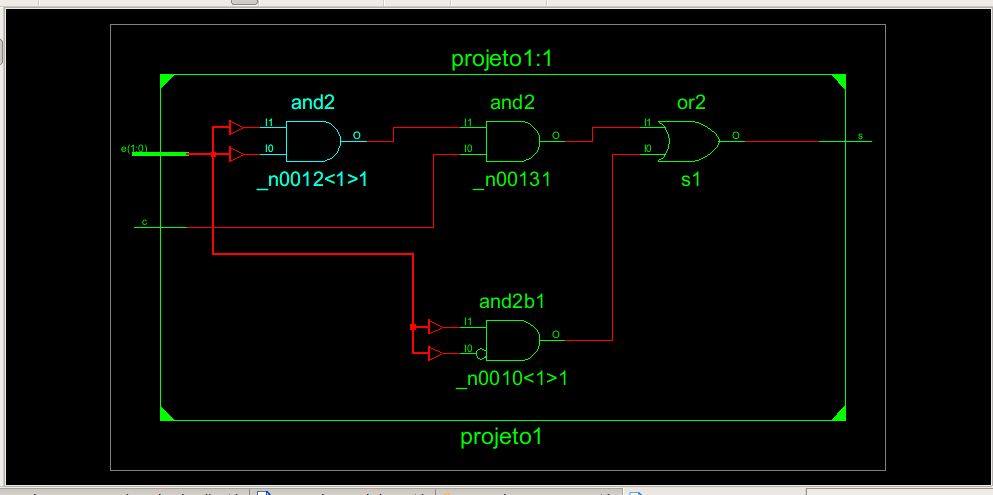
\includegraphics[scale=0.45]{imagens/circuito1}
  \caption{Esquemático projeto 1- Ise Design Suite 14.7}	
  \label{figRotulo}
\end{figure}

\newpage
\subsection{Diagrama de Onda}

\begin{figure}[!htb]
  \centering
  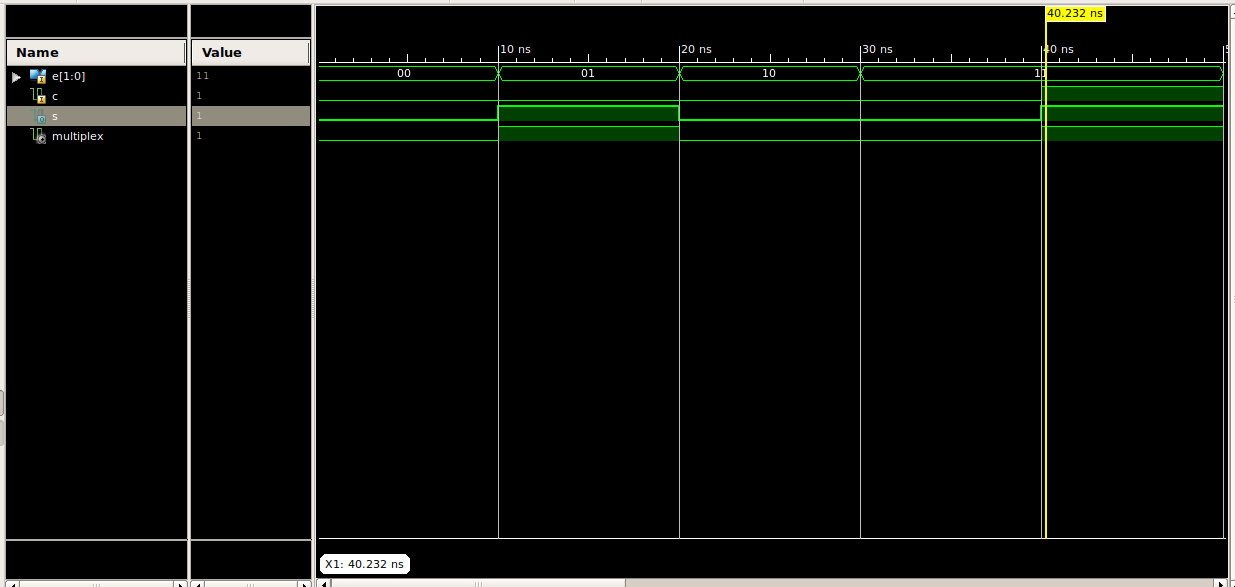
\includegraphics[scale=0.35]{imagens/onda1}
  \caption{Diagrama de ondas projeto 1- Ise Design Suite 14.7}
  \label{figRotulo}
\end{figure}
\newpage

\subsection{Experimento 02}
	O segundo experimento tratou-se de projetar e simular um circuito que implemente a mesma função do experiemnto 01. Utilizando um Demux:2, Mux:2 e uma porta OR.

\clearpage
\subsection{Código VHDL}
\lstinputlisting[language=vhdl]{projetos/projeto2/projeto2.vhd}

\clearpage
\subsection{Diagrama Esquemático versão 1}
\begin{figure}[!htb]
  \centering
  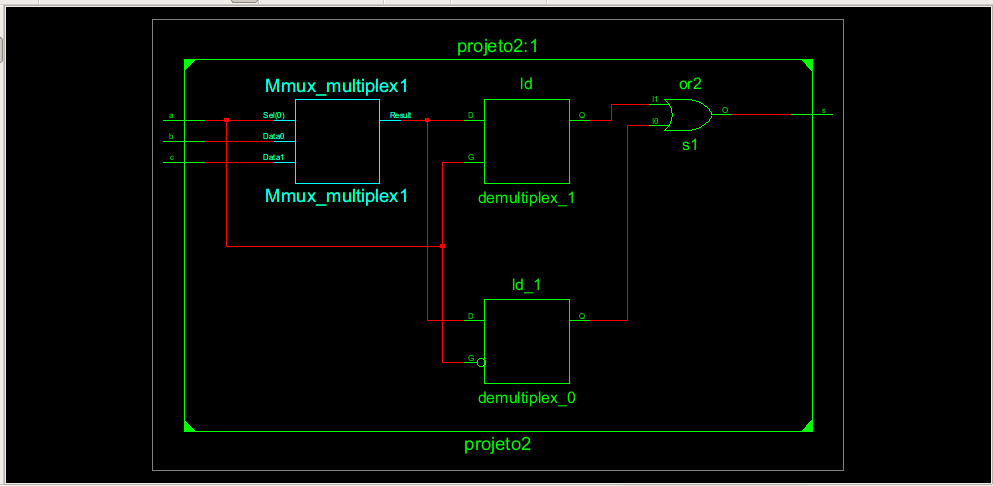
\includegraphics[scale=0.45]{imagens/esquematico2}
  \caption{Esquemático projeto 2 V1 - Ise Design Suite 14.7}	
  \label{figRotulo}
\end{figure}

\newpage
\subsection{Diagrama Esquemático versão 2}
\begin{figure}[!htb]
  \centering
  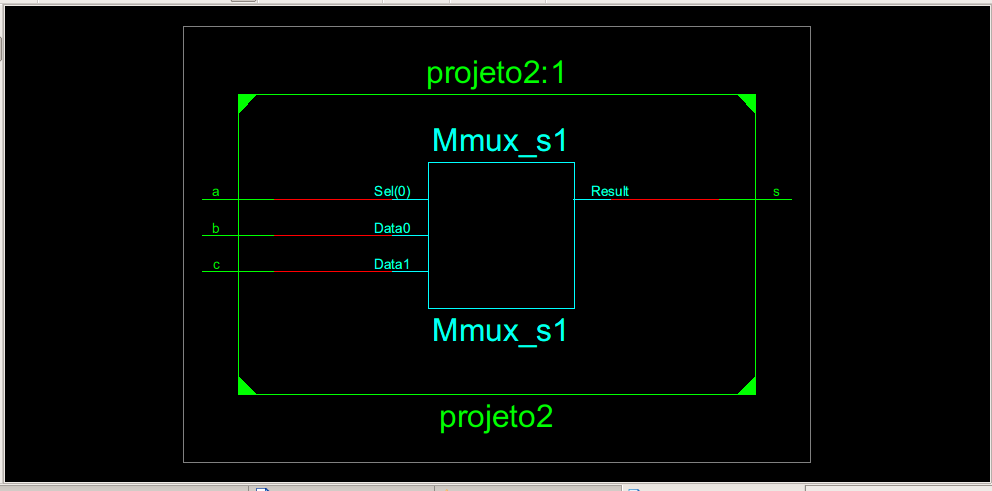
\includegraphics[scale=0.45]{imagens/esquematico22}
  \caption{Esquemático projeto 2 V2 - Ise Design Suite 14.7}	
  \label{figRotulo}
\end{figure}

\subsection{Diagrama de Onda}

\begin{figure}[!htb]
  \centering
  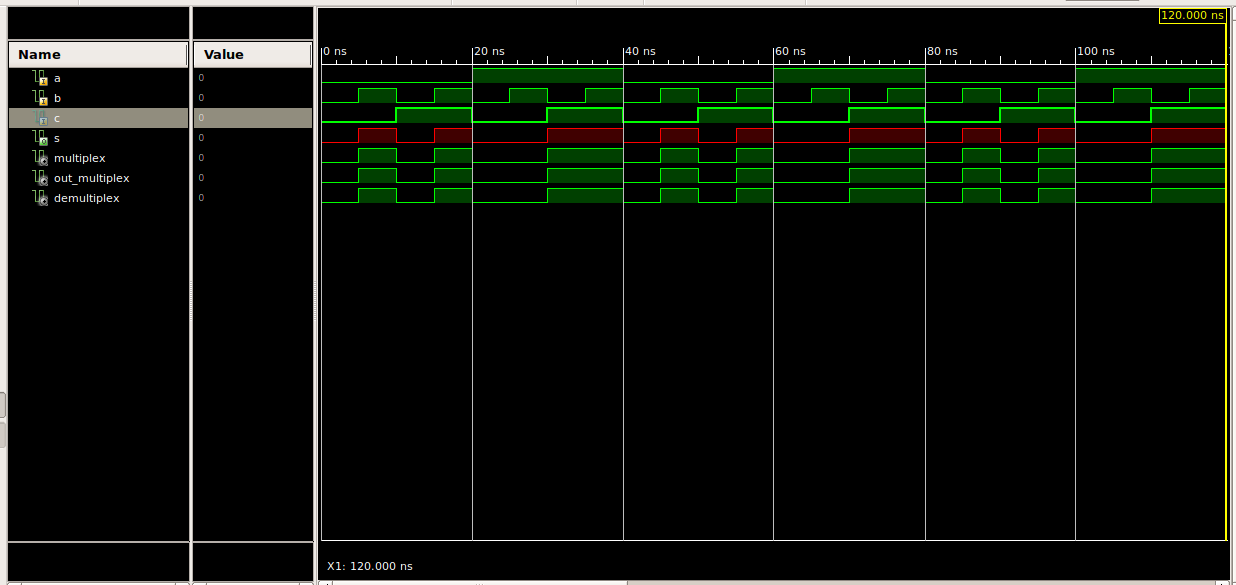
\includegraphics[scale=0.35]{imagens/onda2}
  \caption{Diagrama de ondas Projeto 2 V2 - Ise Design Suite 14.7}
  \label{figRotulo}
\end{figure}
\newpage


\section{Discussão}
\iffalse
Discussão sobre os resultados encontrados, comentando detalhadamente as medições realizadas e dando a devida interpretação destas, informando se os objetivos da experimento foram alcançados. Esta é uma das partes mais importantes do relatório: aqui, há oportunidade para expressar os conhecimentos adquiridos na prática e fazer a interrelação com os fundamentos teóricos.
\fi

        Neste quinto relatório foi possível realizar o primeiro experimento com êxito. Porém, em relação ao segundo experimento tivemos dificuldade na implementação do circuito pois o código em VHDL não correspondia ao resultado esperado quando verificado o diagrama em forma de onda. Para solucionar foi utilizado mais um \textit{signal} e as atribuições para a saida foram feitas fora do \textit{process}.
        
        A solução que alcançou o resultado esperado é a referente à \textbf{versão 2}. Pode-se observar que a implementação do circuito é abstraída para um multiplexador após a implementação do circuito.

\section{Conclusões}
\iffalse
Conclusões, mostrando os êxitos e eventuais problemas encontrados na realização do experimento, indicando as limitações, apresentando recomendações e/ou sugestões.
\fi

Com a realização deste experimento foi possível adquirir conhecimento a respeito de multiplexador e demultiplexador. Suas incríveis funcionalidades e reaproveitamento de circuitos com um auxílio de \textit{clocks}.

\section{Referências Bibliográficas}
\iffalse
Referencias Bibliográficas, relacionadas e citadas de acordo com as normas da ABNT.
\fi
Prática de Eletrônica Digital I 2016.2 professores Henrique Marra Taira Menegaz,Leonardo Aguayo, Lourdes Mattos Brasil, Marcus Vinícius Chaffim Costa, Mariana Costa Bernardes Matias. UnB - FGA Agosto de 2015.

\iffalse
\section{Diagramas Esquemáticos}
Diagramas Esquemáticos. Todos os diagramas devem ser inseridos ao final do relatório em páginas separadas do texto, indicando a identificação do circuito, autor, revisor, versão e datas relevantes.
\fi
\newpage

\end{document}
